\documentclass[1p]{elsarticle_modified}
%\bibliographystyle{elsarticle-num}

%\usepackage[colorlinks]{hyperref}
%\usepackage{abbrmath_seonhwa} %\Abb, \Ascr, \Acal ,\Abf, \Afrak
\usepackage{amsfonts}
\usepackage{amssymb}
\usepackage{amsmath}
\usepackage{amsthm}
\usepackage{scalefnt}
\usepackage{amsbsy}
\usepackage{kotex}
\usepackage{caption}
\usepackage{subfig}
\usepackage{color}
\usepackage{graphicx}
\usepackage{xcolor} %% white, black, red, green, blue, cyan, magenta, yellow
\usepackage{float}
\usepackage{setspace}
\usepackage{hyperref}

\usepackage{tikz}
\usetikzlibrary{arrows}

\usepackage{multirow}
\usepackage{array} % fixed length table
\usepackage{hhline}

%%%%%%%%%%%%%%%%%%%%%
\makeatletter
\renewcommand*\env@matrix[1][\arraystretch]{%
	\edef\arraystretch{#1}%
	\hskip -\arraycolsep
	\let\@ifnextchar\new@ifnextchar
	\array{*\c@MaxMatrixCols c}}
\makeatother %https://tex.stackexchange.com/questions/14071/how-can-i-increase-the-line-spacing-in-a-matrix
%%%%%%%%%%%%%%%

\usepackage[normalem]{ulem}

\newcommand{\msout}[1]{\ifmmode\text{\sout{\ensuremath{#1}}}\else\sout{#1}\fi}
%SOURCE: \msout is \stkout macro in https://tex.stackexchange.com/questions/20609/strikeout-in-math-mode

\newcommand{\cancel}[1]{
	\ifmmode
	{\color{red}\msout{#1}}
	\else
	{\color{red}\sout{#1}}
	\fi
}

\newcommand{\add}[1]{
	{\color{blue}\uwave{#1}}
}

\newcommand{\replace}[2]{
	\ifmmode
	{\color{red}\msout{#1}}{\color{blue}\uwave{#2}}
	\else
	{\color{red}\sout{#1}}{\color{blue}\uwave{#2}}
	\fi
}

\newcommand{\Sol}{\mathcal{S}} %segment
\newcommand{\D}{D} %diagram
\newcommand{\A}{\mathcal{A}} %arc


%%%%%%%%%%%%%%%%%%%%%%%%%%%%%5 test

\def\sl{\operatorname{\textup{SL}}(2,\Cbb)}
\def\psl{\operatorname{\textup{PSL}}(2,\Cbb)}
\def\quan{\mkern 1mu \triangleright \mkern 1mu}

\theoremstyle{definition}
\newtheorem{thm}{Theorem}[section]
\newtheorem{prop}[thm]{Proposition}
\newtheorem{lem}[thm]{Lemma}
\newtheorem{ques}[thm]{Question}
\newtheorem{cor}[thm]{Corollary}
\newtheorem{defn}[thm]{Definition}
\newtheorem{exam}[thm]{Example}
\newtheorem{rmk}[thm]{Remark}
\newtheorem{alg}[thm]{Algorithm}

\newcommand{\I}{\sqrt{-1}}
\begin{document}

%\begin{frontmatter}
%
%\title{Boundary parabolic representations of knots up to 8 crossings}
%
%%% Group authors per affiliation:
%\author{Yunhi Cho} 
%\address{Department of Mathematics, University of Seoul, Seoul, Korea}
%\ead{yhcho@uos.ac.kr}
%
%
%\author{Seonhwa Kim} %\fnref{s_kim}}
%\address{Center for Geometry and Physics, Institute for Basic Science, Pohang, 37673, Korea}
%\ead{ryeona17@ibs.re.kr}
%
%\author{Hyuk Kim}
%\address{Department of Mathematical Sciences, Seoul National University, Seoul 08826, Korea}
%\ead{hyukkim@snu.ac.kr}
%
%\author{Seokbeom Yoon}
%\address{Department of Mathematical Sciences, Seoul National University, Seoul, 08826,  Korea}
%\ead{sbyoon15@snu.ac.kr}
%
%\begin{abstract}
%We find all boundary parabolic representation of knots up to 8 crossings.
%
%\end{abstract}
%\begin{keyword}
%    \MSC[2010] 57M25 
%\end{keyword}
%
%\end{frontmatter}

%\linenumbers
%\tableofcontents
%
\newcommand\colored[1]{\textcolor{white}{\rule[-0.35ex]{0.8em}{1.4ex}}\kern-0.8em\color{red} #1}%
%\newcommand\colored[1]{\textcolor{white}{ #1}\kern-2.17ex	\textcolor{white}{ #1}\kern-1.81ex	\textcolor{white}{ #1}\kern-2.15ex\color{red}#1	}

{\Large $\underline{11a_{78}~(K11a_{78})}$}

\setlength{\tabcolsep}{10pt}
\renewcommand{\arraystretch}{1.6}
\vspace{1cm}\begin{tabular}{m{100pt}>{\centering\arraybackslash}m{274pt}}
\multirow{5}{120pt}{
	\centering
	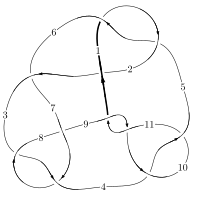
\includegraphics[width=112pt]{../../../GIT/diagram.site/Diagrams/png/327_11a_78.png}\\
\ \ \ A knot diagram\footnotemark}&
\allowdisplaybreaks
\textbf{Linearized knot diagam} \\
\cline{2-2}
 &
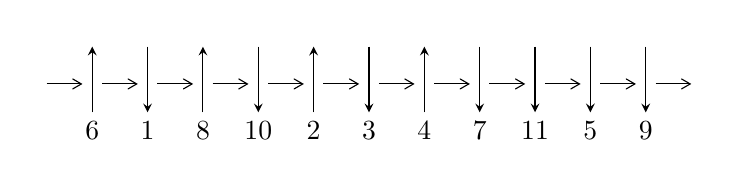
\begin{tikzpicture}[x=20pt, y=17pt]
	% nodes
	\node (C0) at (0, 0) {};
	\node (C1) at (1, 0) {};
	\node (C1U) at (1, +1) {};
	\node (C1D) at (1, -1) {6};

	\node (C2) at (2, 0) {};
	\node (C2U) at (2, +1) {};
	\node (C2D) at (2, -1) {1};

	\node (C3) at (3, 0) {};
	\node (C3U) at (3, +1) {};
	\node (C3D) at (3, -1) {8};

	\node (C4) at (4, 0) {};
	\node (C4U) at (4, +1) {};
	\node (C4D) at (4, -1) {10};

	\node (C5) at (5, 0) {};
	\node (C5U) at (5, +1) {};
	\node (C5D) at (5, -1) {2};

	\node (C6) at (6, 0) {};
	\node (C6U) at (6, +1) {};
	\node (C6D) at (6, -1) {3};

	\node (C7) at (7, 0) {};
	\node (C7U) at (7, +1) {};
	\node (C7D) at (7, -1) {4};

	\node (C8) at (8, 0) {};
	\node (C8U) at (8, +1) {};
	\node (C8D) at (8, -1) {7};

	\node (C9) at (9, 0) {};
	\node (C9U) at (9, +1) {};
	\node (C9D) at (9, -1) {11};

	\node (C10) at (10, 0) {};
	\node (C10U) at (10, +1) {};
	\node (C10D) at (10, -1) {5};

	\node (C11) at (11, 0) {};
	\node (C11U) at (11, +1) {};
	\node (C11D) at (11, -1) {9};
	\node (C12) at (12, 0) {};

	% arrows
	\draw[->,>={angle 60}]
	(C0) edge (C1) (C1) edge (C2) (C2) edge (C3) (C3) edge (C4) (C4) edge (C5) (C5) edge (C6) (C6) edge (C7) (C7) edge (C8) (C8) edge (C9) (C9) edge (C10) (C10) edge (C11) (C11) edge (C12) ;	\draw[->,>=stealth]
	(C1D) edge (C1U) (C2U) edge (C2D) (C3D) edge (C3U) (C4U) edge (C4D) (C5D) edge (C5U) (C6U) edge (C6D) (C7D) edge (C7U) (C8U) edge (C8D) (C9U) edge (C9D) (C10U) edge (C10D) (C11U) edge (C11D) ;
	\end{tikzpicture} \\
\hhline{~~} \\& 
\textbf{Solving Sequence} \\ \cline{2-2} 
 &
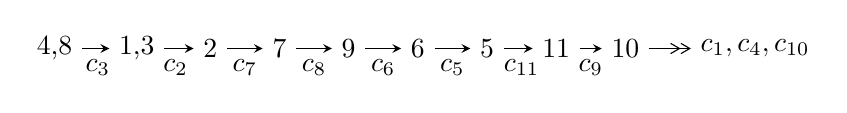
\begin{tikzpicture}[x=25pt, y=7pt]
	% node
	\node (A0) at (-1/8, 0) {4,8};
	\node (A1) at (17/16, 0) {1,3};
	\node (A2) at (17/8, 0) {2};
	\node (A3) at (25/8, 0) {7};
	\node (A4) at (33/8, 0) {9};
	\node (A5) at (41/8, 0) {6};
	\node (A6) at (49/8, 0) {5};
	\node (A7) at (57/8, 0) {11};
	\node (A8) at (65/8, 0) {10};
	\node (C1) at (1/2, -1) {$c_{3}$};
	\node (C2) at (13/8, -1) {$c_{2}$};
	\node (C3) at (21/8, -1) {$c_{7}$};
	\node (C4) at (29/8, -1) {$c_{8}$};
	\node (C5) at (37/8, -1) {$c_{6}$};
	\node (C6) at (45/8, -1) {$c_{5}$};
	\node (C7) at (53/8, -1) {$c_{11}$};
	\node (C8) at (61/8, -1) {$c_{9}$};
	\node (A9) at (10, 0) {$c_{1},c_{4},c_{10}$};

	% edge
	\draw[->,>=stealth]	
	(A0) edge (A1) (A1) edge (A2) (A2) edge (A3) (A3) edge (A4) (A4) edge (A5) (A5) edge (A6) (A6) edge (A7) (A7) edge (A8) ;
	\draw[->>,>={angle 60}]	
	(A8) edge (A9);
\end{tikzpicture} \\ 

\end{tabular} \\

\footnotetext{
The image of knot diagram is generated by the software ``\textbf{Draw programme}" developed by Andrew Bartholomew(\url{http://www.layer8.co.uk/maths/draw/index.htm\#Running-draw}), where we modified some parts for our purpose(\url{https://github.com/CATsTAILs/LinksPainter}).
}\phantom \\ \newline 
\centering \textbf{Ideals for irreducible components\footnotemark of $X_{\text{par}}$} 
 
\begin{align*}
I^u_{1}&=\langle 
u^{24}- u^{23}+\cdots+4 b+1,\;- u^{24}+u^{23}+\cdots+4 a-5,\;u^{25}+6 u^{23}+\cdots+u-1\rangle \\
I^u_{2}&=\langle 
-4476694012 u^{39}-10696306396 u^{38}+\cdots+7868062579 b+9351862960,\\
\phantom{I^u_{2}}&\phantom{= \langle  }-1184460310 u^{39}-263051448 u^{38}+\cdots+605235583 a-1972197779,\;u^{40}+u^{39}+\cdots+2 u+1\rangle \\
I^u_{3}&=\langle 
b+a+1,\;a^2- a u+2 a- u,\;u^2+1\rangle \\
\\
\end{align*}
\raggedright * 3 irreducible components of $\dim_{\mathbb{C}}=0$, with total 69 representations.\\
\footnotetext{All coefficients of polynomials are rational numbers. But the coefficients are sometimes approximated in decimal forms when there is not enough margin.}
\newpage
\renewcommand{\arraystretch}{1}
\centering \section*{I. $I^u_{1}= \langle u^{24}- u^{23}+\cdots+4 b+1,\;- u^{24}+u^{23}+\cdots+4 a-5,\;u^{25}+6 u^{23}+\cdots+u-1 \rangle$}
\flushleft \textbf{(i) Arc colorings}\\
\begin{tabular}{m{7pt} m{180pt} m{7pt} m{180pt} }
\flushright $a_{4}=$&$\begin{pmatrix}1\\0\end{pmatrix}$ \\
\flushright $a_{8}=$&$\begin{pmatrix}0\\u\end{pmatrix}$ \\
\flushright $a_{1}=$&$\begin{pmatrix}\frac{1}{4} u^{24}-\frac{1}{4} u^{23}+\cdots-\frac{1}{2} u+\frac{5}{4}\\-\frac{1}{4} u^{24}+\frac{1}{4} u^{23}+\cdots+\frac{1}{2} u-\frac{1}{4}\end{pmatrix}$ \\
\flushright $a_{3}=$&$\begin{pmatrix}1\\u^2\end{pmatrix}$ \\
\flushright $a_{2}=$&$\begin{pmatrix}\frac{1}{4} u^{24}-\frac{1}{4} u^{23}+\cdots-\frac{1}{2} u+\frac{5}{4}\\-\frac{1}{4} u^{24}+\frac{1}{4} u^{23}+\cdots+\frac{1}{2} u-\frac{1}{4}\end{pmatrix}$ \\
\flushright $a_{7}=$&$\begin{pmatrix}- u\\u\end{pmatrix}$ \\
\flushright $a_{9}=$&$\begin{pmatrix}- u^3\\u^3+u\end{pmatrix}$ \\
\flushright $a_{6}=$&$\begin{pmatrix}u^3\\u^5+u^3+u\end{pmatrix}$ \\
\flushright $a_{5}=$&$\begin{pmatrix}\frac{1}{4} u^{24}+\frac{1}{4} u^{23}+\cdots- u-\frac{1}{4}\\-\frac{1}{4} u^{24}-\frac{1}{4} u^{23}+\cdots+u+\frac{1}{4}\end{pmatrix}$ \\
\flushright $a_{11}=$&$\begin{pmatrix}\frac{1}{2} u^{24}-\frac{1}{2} u^{23}+\cdots- u+\frac{3}{2}\\-\frac{1}{4} u^{24}+\frac{1}{4} u^{23}+\cdots+\frac{1}{2} u-\frac{1}{4}\end{pmatrix}$ \\
\flushright $a_{10}=$&$\begin{pmatrix}\frac{5}{4} u^{24}+\frac{5}{4} u^{23}+\cdots- u-\frac{9}{4}\\-\frac{1}{2} u^{24}-\frac{1}{2} u^{23}+\cdots+u+1\end{pmatrix}$\\ \flushright $a_{10}=$&$\begin{pmatrix}\frac{5}{4} u^{24}+\frac{5}{4} u^{23}+\cdots- u-\frac{9}{4}\\-\frac{1}{2} u^{24}-\frac{1}{2} u^{23}+\cdots+u+1\end{pmatrix}$\\&\end{tabular}
\flushleft \textbf{(ii) Obstruction class $= -1$}\\~\\
\flushleft \textbf{(iii) Cusp Shapes $= -3 u^{24}+u^{23}-18 u^{22}+11 u^{21}-60 u^{20}+44 u^{19}-127 u^{18}+110 u^{17}-194 u^{16}+179 u^{15}-221 u^{14}+213 u^{13}-204 u^{12}+178 u^{11}-159 u^{10}+120 u^9-111 u^8+65 u^7-70 u^6+53 u^5-34 u^4+32 u^3-17 u^2+10 u-8$}\\~\\
\newpage\renewcommand{\arraystretch}{1}
\flushleft \textbf{(iv) u-Polynomials at the component}\newline \\
\begin{tabular}{m{50pt}|m{274pt}}
Crossings & \hspace{64pt}u-Polynomials at each crossing \\
\hline $$\begin{aligned}c_{1},c_{3},c_{5}\\c_{7}\end{aligned}$$&$\begin{aligned}
&u^{25}+6 u^{23}+\cdots+u+1
\end{aligned}$\\
\hline $$\begin{aligned}c_{2},c_{8}\end{aligned}$$&$\begin{aligned}
&u^{25}+12 u^{24}+\cdots-5 u-1
\end{aligned}$\\
\hline $$\begin{aligned}c_{4},c_{10}\end{aligned}$$&$\begin{aligned}
&u^{25}-3 u^{24}+\cdots-5 u+2
\end{aligned}$\\
\hline $$\begin{aligned}c_{6}\end{aligned}$$&$\begin{aligned}
&u^{25}+3 u^{24}+\cdots+16 u+32
\end{aligned}$\\
\hline $$\begin{aligned}c_{9},c_{11}\end{aligned}$$&$\begin{aligned}
&u^{25}+9 u^{24}+\cdots-7 u+4
\end{aligned}$\\
\hline
\end{tabular}\\~\\
\newpage\renewcommand{\arraystretch}{1}
\flushleft \textbf{(v) Riley Polynomials at the component}\newline \\
\begin{tabular}{m{50pt}|m{274pt}}
Crossings & \hspace{64pt}Riley Polynomials at each crossing \\
\hline $$\begin{aligned}c_{1},c_{3},c_{5}\\c_{7}\end{aligned}$$&$\begin{aligned}
&y^{25}+12 y^{24}+\cdots-5 y-1
\end{aligned}$\\
\hline $$\begin{aligned}c_{2},c_{8}\end{aligned}$$&$\begin{aligned}
&y^{25}+8 y^{24}+\cdots+3 y-1
\end{aligned}$\\
\hline $$\begin{aligned}c_{4},c_{10}\end{aligned}$$&$\begin{aligned}
&y^{25}-9 y^{24}+\cdots-7 y-4
\end{aligned}$\\
\hline $$\begin{aligned}c_{6}\end{aligned}$$&$\begin{aligned}
&y^{25}-11 y^{24}+\cdots-13568 y-1024
\end{aligned}$\\
\hline $$\begin{aligned}c_{9},c_{11}\end{aligned}$$&$\begin{aligned}
&y^{25}+15 y^{24}+\cdots+273 y-16
\end{aligned}$\\
\hline
\end{tabular}\\~\\
\newpage\flushleft \textbf{(vi) Complex Volumes and Cusp Shapes}
$$\begin{array}{c|c|c}  
\text{Solutions to }I^u_{1}& \I (\text{vol} + \sqrt{-1}CS) & \text{Cusp shape}\\
 \hline 
\begin{aligned}
u &= -0.668066 + 0.826958 I \\
a &= -0.391410 + 0.121275 I \\
b &= -0.010569 - 0.701256 I\end{aligned}
 & \phantom{-}4.42357 - 2.28876 I & \phantom{-}0.90025 + 3.22916 I \\ \hline\begin{aligned}
u &= -0.668066 - 0.826958 I \\
a &= -0.391410 - 0.121275 I \\
b &= -0.010569 + 0.701256 I\end{aligned}
 & \phantom{-}4.42357 + 2.28876 I & \phantom{-}0.90025 - 3.22916 I \\ \hline\begin{aligned}
u &= \phantom{-}0.387315 + 0.828510 I \\
a &= -0.057213 - 1.406030 I \\
b &= \phantom{-}0.39665 + 1.35928 I\end{aligned}
 & -2.29786 + 4.38512 I & -6.23003 - 9.05656 I \\ \hline\begin{aligned}
u &= \phantom{-}0.387315 - 0.828510 I \\
a &= -0.057213 + 1.406030 I \\
b &= \phantom{-}0.39665 - 1.35928 I\end{aligned}
 & -2.29786 - 4.38512 I & -6.23003 + 9.05656 I \\ \hline\begin{aligned}
u &= \phantom{-}0.663122 + 0.885711 I \\
a &= -0.620402 - 0.123885 I \\
b &= \phantom{-}0.014657 + 0.488612 I\end{aligned}
 & \phantom{-}4.05826 + 8.02736 I & -0.26249 - 8.69949 I \\ \hline\begin{aligned}
u &= \phantom{-}0.663122 - 0.885711 I \\
a &= -0.620402 + 0.123885 I \\
b &= \phantom{-}0.014657 - 0.488612 I\end{aligned}
 & \phantom{-}4.05826 - 8.02736 I & -0.26249 + 8.69949 I \\ \hline\begin{aligned}
u &= \phantom{-}0.781060 + 0.295309 I \\
a &= \phantom{-}0.725790 + 0.096907 I \\
b &= \phantom{-}0.857621 + 0.846789 I\end{aligned}
 & \phantom{-}2.49934 - 5.05647 I & \phantom{-}0.76088 + 3.39553 I \\ \hline\begin{aligned}
u &= \phantom{-}0.781060 - 0.295309 I \\
a &= \phantom{-}0.725790 - 0.096907 I \\
b &= \phantom{-}0.857621 - 0.846789 I\end{aligned}
 & \phantom{-}2.49934 + 5.05647 I & \phantom{-}0.76088 - 3.39553 I \\ \hline\begin{aligned}
u &= -0.732724 + 0.365786 I \\
a &= \phantom{-}0.646963 - 0.060825 I \\
b &= \phantom{-}0.631263 - 0.907356 I\end{aligned}
 & \phantom{-}3.32057 - 0.44324 I & \phantom{-}2.54503 + 2.33373 I \\ \hline\begin{aligned}
u &= -0.732724 - 0.365786 I \\
a &= \phantom{-}0.646963 + 0.060825 I \\
b &= \phantom{-}0.631263 + 0.907356 I\end{aligned}
 & \phantom{-}3.32057 + 0.44324 I & \phantom{-}2.54503 - 2.33373 I\\
 \hline 
 \end{array}$$\newpage$$\begin{array}{c|c|c}  
\text{Solutions to }I^u_{1}& \I (\text{vol} + \sqrt{-1}CS) & \text{Cusp shape}\\
 \hline 
\begin{aligned}
u &= -0.440401 + 1.120690 I \\
a &= -2.18870 + 1.03108 I \\
b &= \phantom{-}2.28016 + 0.07839 I\end{aligned}
 & -4.91803 - 1.59228 I & -7.91949 + 2.30620 I \\ \hline\begin{aligned}
u &= -0.440401 - 1.120690 I \\
a &= -2.18870 - 1.03108 I \\
b &= \phantom{-}2.28016 - 0.07839 I\end{aligned}
 & -4.91803 + 1.59228 I & -7.91949 - 2.30620 I \\ \hline\begin{aligned}
u &= \phantom{-}0.496157 + 1.112700 I \\
a &= -1.97870 - 0.70710 I \\
b &= \phantom{-}1.75155 - 0.37924 I\end{aligned}
 & -2.95653 + 6.50680 I & -4.30037 - 6.80019 I \\ \hline\begin{aligned}
u &= \phantom{-}0.496157 - 1.112700 I \\
a &= -1.97870 + 0.70710 I \\
b &= \phantom{-}1.75155 + 0.37924 I\end{aligned}
 & -2.95653 - 6.50680 I & -4.30037 + 6.80019 I \\ \hline\begin{aligned}
u &= -0.447856 + 0.612567 I \\
a &= \phantom{-}0.505867 + 0.568532 I \\
b &= \phantom{-}0.048924 - 0.925546 I\end{aligned}
 & \phantom{-}0.53657 - 1.46473 I & \phantom{-}1.57744 + 4.49882 I \\ \hline\begin{aligned}
u &= -0.447856 - 0.612567 I \\
a &= \phantom{-}0.505867 - 0.568532 I \\
b &= \phantom{-}0.048924 + 0.925546 I\end{aligned}
 & \phantom{-}0.53657 + 1.46473 I & \phantom{-}1.57744 - 4.49882 I \\ \hline\begin{aligned}
u &= -0.502100 + 1.180640 I \\
a &= -2.34071 + 0.47753 I \\
b &= \phantom{-}2.09699 + 1.04430 I\end{aligned}
 & -8.02282 - 8.65791 I & -10.60850 + 6.91846 I \\ \hline\begin{aligned}
u &= -0.502100 - 1.180640 I \\
a &= -2.34071 - 0.47753 I \\
b &= \phantom{-}2.09699 - 1.04430 I\end{aligned}
 & -8.02282 + 8.65791 I & -10.60850 - 6.91846 I \\ \hline\begin{aligned}
u &= \phantom{-}0.562594 + 1.178700 I \\
a &= -2.15539 - 0.17720 I \\
b &= \phantom{-}1.47455 - 1.34225 I\end{aligned}
 & -1.63771 + 9.61928 I & -3.84139 - 5.85883 I \\ \hline\begin{aligned}
u &= \phantom{-}0.562594 - 1.178700 I \\
a &= -2.15539 + 0.17720 I \\
b &= \phantom{-}1.47455 + 1.34225 I\end{aligned}
 & -1.63771 - 9.61928 I & -3.84139 + 5.85883 I\\
 \hline 
 \end{array}$$\newpage$$\begin{array}{c|c|c}  
\text{Solutions to }I^u_{1}& \I (\text{vol} + \sqrt{-1}CS) & \text{Cusp shape}\\
 \hline 
\begin{aligned}
u &= \phantom{-}0.147311 + 0.674791 I \\
a &= \phantom{-}1.71030 - 0.90481 I \\
b &= -0.995418 + 0.931192 I\end{aligned}
 & -1.78656 - 1.53483 I & -3.61707 + 0.13208 I \\ \hline\begin{aligned}
u &= \phantom{-}0.147311 - 0.674791 I \\
a &= \phantom{-}1.71030 + 0.90481 I \\
b &= -0.995418 - 0.931192 I\end{aligned}
 & -1.78656 + 1.53483 I & -3.61707 - 0.13208 I \\ \hline\begin{aligned}
u &= -0.562275 + 1.202520 I \\
a &= -2.27068 + 0.11315 I \\
b &= \phantom{-}1.58876 + 1.59048 I\end{aligned}
 & -2.9757 - 15.3316 I & -5.87847 + 10.26197 I \\ \hline\begin{aligned}
u &= -0.562275 - 1.202520 I \\
a &= -2.27068 - 0.11315 I \\
b &= \phantom{-}1.58876 - 1.59048 I\end{aligned}
 & -2.9757 + 15.3316 I & -5.87847 - 10.26197 I \\ \hline\begin{aligned}
u &= \phantom{-}0.631724\phantom{ +0.000000I} \\
a &= \phantom{-}0.828591\phantom{ +0.000000I} \\
b &= \phantom{-}0.729746\phantom{ +0.000000I}\end{aligned}
 & -1.87036\phantom{ +0.000000I} & -4.25160\phantom{ +0.000000I}\\
 \hline 
 \end{array}$$\newpage\newpage\renewcommand{\arraystretch}{1}
\centering \section*{II. $I^u_{2}= \langle -4.48\times10^{9} u^{39}-1.07\times10^{10} u^{38}+\cdots+7.87\times10^{9} b+9.35\times10^{9},\;-1.18\times10^{9} u^{39}-2.63\times10^{8} u^{38}+\cdots+6.05\times10^{8} a-1.97\times10^{9},\;u^{40}+u^{39}+\cdots+2 u+1 \rangle$}
\flushleft \textbf{(i) Arc colorings}\\
\begin{tabular}{m{7pt} m{180pt} m{7pt} m{180pt} }
\flushright $a_{4}=$&$\begin{pmatrix}1\\0\end{pmatrix}$ \\
\flushright $a_{8}=$&$\begin{pmatrix}0\\u\end{pmatrix}$ \\
\flushright $a_{1}=$&$\begin{pmatrix}1.95702 u^{39}+0.434627 u^{38}+\cdots-0.306306 u+3.25856\\0.568970 u^{39}+1.35946 u^{38}+\cdots+0.868382 u-1.18859\end{pmatrix}$ \\
\flushright $a_{3}=$&$\begin{pmatrix}1\\u^2\end{pmatrix}$ \\
\flushright $a_{2}=$&$\begin{pmatrix}2.52599 u^{39}+1.79409 u^{38}+\cdots+0.562076 u+3.06998\\-1.08110 u^{39}-0.476540 u^{38}+\cdots-0.632572 u-3.87864\end{pmatrix}$ \\
\flushright $a_{7}=$&$\begin{pmatrix}- u\\u\end{pmatrix}$ \\
\flushright $a_{9}=$&$\begin{pmatrix}- u^3\\u^3+u\end{pmatrix}$ \\
\flushright $a_{6}=$&$\begin{pmatrix}u^3\\u^5+u^3+u\end{pmatrix}$ \\
\flushright $a_{5}=$&$\begin{pmatrix}-1.92049 u^{39}-1.64843 u^{38}+\cdots-4.76213 u-5.77155\\-2.08550 u^{39}-1.17361 u^{38}+\cdots-1.60565 u-2.79806\end{pmatrix}$ \\
\flushright $a_{11}=$&$\begin{pmatrix}2.26791 u^{39}-0.119746 u^{38}+\cdots-1.61688 u+3.05922\\-0.653801 u^{39}+0.802602 u^{38}+\cdots+0.806017 u-3.07474\end{pmatrix}$ \\
\flushright $a_{10}=$&$\begin{pmatrix}-2.49055 u^{39}-0.832197 u^{38}+\cdots-2.76553 u-7.09778\\-1.67912 u^{39}-1.52806 u^{38}+\cdots-2.35663 u-1.41907\end{pmatrix}$\\ \flushright $a_{10}=$&$\begin{pmatrix}-2.49055 u^{39}-0.832197 u^{38}+\cdots-2.76553 u-7.09778\\-1.67912 u^{39}-1.52806 u^{38}+\cdots-2.35663 u-1.41907\end{pmatrix}$\\&\end{tabular}
\flushleft \textbf{(ii) Obstruction class $= -1$}\\~\\
\flushleft \textbf{(iii) Cusp Shapes $= -\frac{51184596416}{7868062579} u^{39}-\frac{71297250008}{7868062579} u^{38}+\cdots-\frac{117349868140}{7868062579} u-\frac{113505824050}{7868062579}$}\\~\\
\newpage\renewcommand{\arraystretch}{1}
\flushleft \textbf{(iv) u-Polynomials at the component}\newline \\
\begin{tabular}{m{50pt}|m{274pt}}
Crossings & \hspace{64pt}u-Polynomials at each crossing \\
\hline $$\begin{aligned}c_{1},c_{3},c_{5}\\c_{7}\end{aligned}$$&$\begin{aligned}
&u^{40}- u^{39}+\cdots-2 u+1
\end{aligned}$\\
\hline $$\begin{aligned}c_{2},c_{8}\end{aligned}$$&$\begin{aligned}
&u^{40}+23 u^{39}+\cdots-16 u^2+1
\end{aligned}$\\
\hline $$\begin{aligned}c_{4},c_{10}\end{aligned}$$&$\begin{aligned}
&(u^{20}+u^{19}+\cdots+3 u^2-1)^{2}
\end{aligned}$\\
\hline $$\begin{aligned}c_{6}\end{aligned}$$&$\begin{aligned}
&(u^{20}- u^{19}+\cdots+4 u-1)^{2}
\end{aligned}$\\
\hline $$\begin{aligned}c_{9},c_{11}\end{aligned}$$&$\begin{aligned}
&(u^{20}+7 u^{19}+\cdots+6 u+1)^{2}
\end{aligned}$\\
\hline
\end{tabular}\\~\\
\newpage\renewcommand{\arraystretch}{1}
\flushleft \textbf{(v) Riley Polynomials at the component}\newline \\
\begin{tabular}{m{50pt}|m{274pt}}
Crossings & \hspace{64pt}Riley Polynomials at each crossing \\
\hline $$\begin{aligned}c_{1},c_{3},c_{5}\\c_{7}\end{aligned}$$&$\begin{aligned}
&y^{40}+23 y^{39}+\cdots-16 y^2+1
\end{aligned}$\\
\hline $$\begin{aligned}c_{2},c_{8}\end{aligned}$$&$\begin{aligned}
&y^{40}-13 y^{39}+\cdots-32 y+1
\end{aligned}$\\
\hline $$\begin{aligned}c_{4},c_{10}\end{aligned}$$&$\begin{aligned}
&(y^{20}-7 y^{19}+\cdots-6 y+1)^{2}
\end{aligned}$\\
\hline $$\begin{aligned}c_{6}\end{aligned}$$&$\begin{aligned}
&(y^{20}-11 y^{19}+\cdots-6 y+1)^{2}
\end{aligned}$\\
\hline $$\begin{aligned}c_{9},c_{11}\end{aligned}$$&$\begin{aligned}
&(y^{20}+13 y^{19}+\cdots-6 y+1)^{2}
\end{aligned}$\\
\hline
\end{tabular}\\~\\
\newpage\flushleft \textbf{(vi) Complex Volumes and Cusp Shapes}
$$\begin{array}{c|c|c}  
\text{Solutions to }I^u_{2}& \I (\text{vol} + \sqrt{-1}CS) & \text{Cusp shape}\\
 \hline 
\begin{aligned}
u &= -0.680660 + 0.735978 I \\
a &= \phantom{-}1.061240 - 0.028188 I \\
b &= -0.0630213 - 0.1220620 I\end{aligned}
 & \phantom{-}4.68486 - 2.84648 I & \phantom{-}1.60998 + 2.97861 I \\ \hline\begin{aligned}
u &= -0.680660 - 0.735978 I \\
a &= \phantom{-}1.061240 + 0.028188 I \\
b &= -0.0630213 + 0.1220620 I\end{aligned}
 & \phantom{-}4.68486 + 2.84648 I & \phantom{-}1.60998 - 2.97861 I \\ \hline\begin{aligned}
u &= \phantom{-}0.703070 + 0.667774 I \\
a &= \phantom{-}0.935371 + 0.031857 I \\
b &= -0.0630213 - 0.1220620 I\end{aligned}
 & \phantom{-}4.68486 - 2.84648 I & \phantom{-}1.60998 + 2.97861 I \\ \hline\begin{aligned}
u &= \phantom{-}0.703070 - 0.667774 I \\
a &= \phantom{-}0.935371 - 0.031857 I \\
b &= -0.0630213 + 0.1220620 I\end{aligned}
 & \phantom{-}4.68486 + 2.84648 I & \phantom{-}1.60998 - 2.97861 I \\ \hline\begin{aligned}
u &= \phantom{-}0.179409 + 1.047170 I \\
a &= -1.007340 - 0.708627 I \\
b &= \phantom{-}0.274077\phantom{ +0.000000I}\end{aligned}
 & -3.97005\phantom{ +0.000000I} & -10.76209 + 0. I\phantom{ +0.000000I} \\ \hline\begin{aligned}
u &= \phantom{-}0.179409 - 1.047170 I \\
a &= -1.007340 + 0.708627 I \\
b &= \phantom{-}0.274077\phantom{ +0.000000I}\end{aligned}
 & -3.97005\phantom{ +0.000000I} & -10.76209 + 0. I\phantom{ +0.000000I} \\ \hline\begin{aligned}
u &= -0.406752 + 0.984604 I \\
a &= \phantom{-}1.305660 - 0.307787 I \\
b &= -0.994955 - 0.489591 I\end{aligned}
 & -0.52569 - 2.16136 I & -0.73748 + 3.31855 I \\ \hline\begin{aligned}
u &= -0.406752 - 0.984604 I \\
a &= \phantom{-}1.305660 + 0.307787 I \\
b &= -0.994955 + 0.489591 I\end{aligned}
 & -0.52569 + 2.16136 I & -0.73748 - 3.31855 I \\ \hline\begin{aligned}
u &= -0.883398 + 0.214209 I \\
a &= -0.296276 - 0.096762 I \\
b &= -1.25336 + 1.31067 I\end{aligned}
 & -0.00745 + 10.05770 I & -2.70834 - 7.26612 I \\ \hline\begin{aligned}
u &= -0.883398 - 0.214209 I \\
a &= -0.296276 + 0.096762 I \\
b &= -1.25336 - 1.31067 I\end{aligned}
 & -0.00745 - 10.05770 I & -2.70834 + 7.26612 I\\
 \hline 
 \end{array}$$\newpage$$\begin{array}{c|c|c}  
\text{Solutions to }I^u_{2}& \I (\text{vol} + \sqrt{-1}CS) & \text{Cusp shape}\\
 \hline 
\begin{aligned}
u &= \phantom{-}0.847173 + 0.247485 I \\
a &= -0.164766 + 0.157989 I \\
b &= -1.09019 - 1.18394 I\end{aligned}
 & \phantom{-}1.14075 - 4.43308 I & -0.68370 + 2.52728 I \\ \hline\begin{aligned}
u &= \phantom{-}0.847173 - 0.247485 I \\
a &= -0.164766 - 0.157989 I \\
b &= -1.09019 + 1.18394 I\end{aligned}
 & \phantom{-}1.14075 + 4.43308 I & -0.68370 - 2.52728 I \\ \hline\begin{aligned}
u &= \phantom{-}0.240047 + 1.118770 I \\
a &= \phantom{-}1.126200 + 0.481500 I \\
b &= -1.340740 + 0.080597 I\end{aligned}
 & -2.02098 - 2.13456 I & -4.50898 + 2.16962 I \\ \hline\begin{aligned}
u &= \phantom{-}0.240047 - 1.118770 I \\
a &= \phantom{-}1.126200 - 0.481500 I \\
b &= -1.340740 - 0.080597 I\end{aligned}
 & -2.02098 + 2.13456 I & -4.50898 - 2.16962 I \\ \hline\begin{aligned}
u &= \phantom{-}0.416062 + 1.082120 I \\
a &= -1.36848 - 1.28995 I \\
b &= \phantom{-}1.070070 - 0.629261 I\end{aligned}
 & -3.61438 + 0.81573 I & -5.67172 - 1.07888 I \\ \hline\begin{aligned}
u &= \phantom{-}0.416062 - 1.082120 I \\
a &= -1.36848 + 1.28995 I \\
b &= \phantom{-}1.070070 + 0.629261 I\end{aligned}
 & -3.61438 - 0.81573 I & -5.67172 + 1.07888 I \\ \hline\begin{aligned}
u &= -0.017851 + 1.176950 I \\
a &= \phantom{-}0.345233 - 0.405044 I \\
b &= -0.710796 + 0.321114 I\end{aligned}
 & -1.62333 - 2.35832 I & -2.35225 + 4.49783 I \\ \hline\begin{aligned}
u &= -0.017851 - 1.176950 I \\
a &= \phantom{-}0.345233 + 0.405044 I \\
b &= -0.710796 - 0.321114 I\end{aligned}
 & -1.62333 + 2.35832 I & -2.35225 - 4.49783 I \\ \hline\begin{aligned}
u &= -0.460657 + 1.121820 I \\
a &= -1.40263 + 1.43442 I \\
b &= \phantom{-}1.42212 + 0.74562 I\end{aligned}
 & -4.77271 - 6.07240 I & -7.45285 + 5.87540 I \\ \hline\begin{aligned}
u &= -0.460657 - 1.121820 I \\
a &= -1.40263 - 1.43442 I \\
b &= \phantom{-}1.42212 - 0.74562 I\end{aligned}
 & -4.77271 + 6.07240 I & -7.45285 - 5.87540 I\\
 \hline 
 \end{array}$$\newpage$$\begin{array}{c|c|c}  
\text{Solutions to }I^u_{2}& \I (\text{vol} + \sqrt{-1}CS) & \text{Cusp shape}\\
 \hline 
\begin{aligned}
u &= -0.771680 + 0.120837 I \\
a &= -0.436638 - 0.516967 I \\
b &= -1.45055 + 0.79305 I\end{aligned}
 & -4.94645 + 3.96853 I & -7.89349 - 3.79787 I \\ \hline\begin{aligned}
u &= -0.771680 - 0.120837 I \\
a &= -0.436638 + 0.516967 I \\
b &= -1.45055 - 0.79305 I\end{aligned}
 & -4.94645 - 3.96853 I & -7.89349 + 3.79787 I \\ \hline\begin{aligned}
u &= \phantom{-}0.444139 + 1.139190 I \\
a &= \phantom{-}1.44372 + 0.43742 I \\
b &= -1.45055 + 0.79305 I\end{aligned}
 & -4.94645 + 3.96853 I & -7.89349 - 3.79787 I \\ \hline\begin{aligned}
u &= \phantom{-}0.444139 - 1.139190 I \\
a &= \phantom{-}1.44372 - 0.43742 I \\
b &= -1.45055 - 0.79305 I\end{aligned}
 & -4.94645 - 3.96853 I & -7.89349 + 3.79787 I \\ \hline\begin{aligned}
u &= -0.551606 + 1.104560 I \\
a &= \phantom{-}1.52922 - 0.28411 I \\
b &= -1.09019 - 1.18394 I\end{aligned}
 & \phantom{-}1.14075 - 4.43308 I & -0.68370 + 2.52728 I \\ \hline\begin{aligned}
u &= -0.551606 - 1.104560 I \\
a &= \phantom{-}1.52922 + 0.28411 I \\
b &= -1.09019 + 1.18394 I\end{aligned}
 & \phantom{-}1.14075 + 4.43308 I & -0.68370 - 2.52728 I \\ \hline\begin{aligned}
u &= -0.386163 + 1.203070 I \\
a &= -1.11143 + 1.51116 I \\
b &= \phantom{-}1.54877\phantom{ +0.000000I}\end{aligned}
 & -8.84775\phantom{ +0.000000I} & -12.44026 + 0. I\phantom{ +0.000000I} \\ \hline\begin{aligned}
u &= -0.386163 - 1.203070 I \\
a &= -1.11143 - 1.51116 I \\
b &= \phantom{-}1.54877\phantom{ +0.000000I}\end{aligned}
 & -8.84775\phantom{ +0.000000I} & -12.44026 + 0. I\phantom{ +0.000000I} \\ \hline\begin{aligned}
u &= \phantom{-}0.276270 + 1.238300 I \\
a &= -0.75891 - 1.40625 I \\
b &= \phantom{-}1.070070 + 0.629261 I\end{aligned}
 & -3.61438 - 0.81573 I & -5.67172 + 1.07888 I \\ \hline\begin{aligned}
u &= \phantom{-}0.276270 - 1.238300 I \\
a &= -0.75891 + 1.40625 I \\
b &= \phantom{-}1.070070 - 0.629261 I\end{aligned}
 & -3.61438 + 0.81573 I & -5.67172 - 1.07888 I\\
 \hline 
 \end{array}$$\newpage$$\begin{array}{c|c|c}  
\text{Solutions to }I^u_{2}& \I (\text{vol} + \sqrt{-1}CS) & \text{Cusp shape}\\
 \hline 
\begin{aligned}
u &= \phantom{-}0.555192 + 1.143400 I \\
a &= \phantom{-}1.58253 + 0.32035 I \\
b &= -1.25336 + 1.31067 I\end{aligned}
 & -0.00745 + 10.05770 I & -3.00000 - 7.26612 I \\ \hline\begin{aligned}
u &= \phantom{-}0.555192 - 1.143400 I \\
a &= \phantom{-}1.58253 - 0.32035 I \\
b &= -1.25336 - 1.31067 I\end{aligned}
 & -0.00745 - 10.05770 I & -3.00000 + 7.26612 I \\ \hline\begin{aligned}
u &= -0.312447 + 1.274980 I \\
a &= -0.79278 + 1.57779 I \\
b &= \phantom{-}1.42212 - 0.74562 I\end{aligned}
 & -4.77271 + 6.07240 I & -7.45285 - 5.87540 I \\ \hline\begin{aligned}
u &= -0.312447 - 1.274980 I \\
a &= -0.79278 - 1.57779 I \\
b &= \phantom{-}1.42212 + 0.74562 I\end{aligned}
 & -4.77271 - 6.07240 I & -7.45285 + 5.87540 I \\ \hline\begin{aligned}
u &= \phantom{-}0.605286 + 0.255049 I \\
a &= \phantom{-}0.207408 + 0.820889 I \\
b &= -0.994955 - 0.489591 I\end{aligned}
 & -0.52569 - 2.16136 I & -0.73748 + 3.31855 I \\ \hline\begin{aligned}
u &= \phantom{-}0.605286 - 0.255049 I \\
a &= \phantom{-}0.207408 - 0.820889 I \\
b &= -0.994955 + 0.489591 I\end{aligned}
 & -0.52569 + 2.16136 I & -0.73748 - 3.31855 I \\ \hline\begin{aligned}
u &= \phantom{-}0.219360 + 0.513597 I \\
a &= -2.33551 - 0.75634 I \\
b &= -0.710796 - 0.321114 I\end{aligned}
 & -1.62333 + 2.35832 I & -2.35225 - 4.49783 I \\ \hline\begin{aligned}
u &= \phantom{-}0.219360 - 0.513597 I \\
a &= -2.33551 + 0.75634 I \\
b &= -0.710796 + 0.321114 I\end{aligned}
 & -1.62333 - 2.35832 I & -2.35225 + 4.49783 I \\ \hline\begin{aligned}
u &= -0.514794 + 0.049169 I \\
a &= -0.86181 + 1.57235 I \\
b &= -1.340740 - 0.080597 I\end{aligned}
 & -2.02098 + 2.13456 I & -4.50898 - 2.16962 I \\ \hline\begin{aligned}
u &= -0.514794 - 0.049169 I \\
a &= -0.86181 - 1.57235 I \\
b &= -1.340740 + 0.080597 I\end{aligned}
 & -2.02098 - 2.13456 I & -4.50898 + 2.16962 I\\
 \hline 
 \end{array}$$\newpage\newpage\renewcommand{\arraystretch}{1}
\centering \section*{III. $I^u_{3}= \langle b+a+1,\;a^2- a u+2 a- u,\;u^2+1 \rangle$}
\flushleft \textbf{(i) Arc colorings}\\
\begin{tabular}{m{7pt} m{180pt} m{7pt} m{180pt} }
\flushright $a_{4}=$&$\begin{pmatrix}1\\0\end{pmatrix}$ \\
\flushright $a_{8}=$&$\begin{pmatrix}0\\u\end{pmatrix}$ \\
\flushright $a_{1}=$&$\begin{pmatrix}a\\- a-1\end{pmatrix}$ \\
\flushright $a_{3}=$&$\begin{pmatrix}1\\-1\end{pmatrix}$ \\
\flushright $a_{2}=$&$\begin{pmatrix}a+1\\- a-2\end{pmatrix}$ \\
\flushright $a_{7}=$&$\begin{pmatrix}- u\\u\end{pmatrix}$ \\
\flushright $a_{9}=$&$\begin{pmatrix}u\\0\end{pmatrix}$ \\
\flushright $a_{6}=$&$\begin{pmatrix}- u\\u\end{pmatrix}$ \\
\flushright $a_{5}=$&$\begin{pmatrix}a u\\- a u- u\end{pmatrix}$ \\
\flushright $a_{11}=$&$\begin{pmatrix}2 a+1\\- a-1\end{pmatrix}$ \\
\flushright $a_{10}=$&$\begin{pmatrix}a u+2 a+2\\- a+u-1\end{pmatrix}$\\ \flushright $a_{10}=$&$\begin{pmatrix}a u+2 a+2\\- a+u-1\end{pmatrix}$\\&\end{tabular}
\flushleft \textbf{(ii) Obstruction class $= 1$}\\~\\
\flushleft \textbf{(iii) Cusp Shapes $= -4 a u-4 u-12$}\\~\\
\newpage\renewcommand{\arraystretch}{1}
\flushleft \textbf{(iv) u-Polynomials at the component}\newline \\
\begin{tabular}{m{50pt}|m{274pt}}
Crossings & \hspace{64pt}u-Polynomials at each crossing \\
\hline $$\begin{aligned}c_{1},c_{3},c_{5}\\c_{7}\end{aligned}$$&$\begin{aligned}
&(u^2+1)^2
\end{aligned}$\\
\hline $$\begin{aligned}c_{2},c_{8}\end{aligned}$$&$\begin{aligned}
&(u+1)^4
\end{aligned}$\\
\hline $$\begin{aligned}c_{4},c_{10}\end{aligned}$$&$\begin{aligned}
&u^4- u^2+1
\end{aligned}$\\
\hline $$\begin{aligned}c_{6}\end{aligned}$$&$\begin{aligned}
&u^4
\end{aligned}$\\
\hline $$\begin{aligned}c_{9}\end{aligned}$$&$\begin{aligned}
&(u^2- u+1)^2
\end{aligned}$\\
\hline $$\begin{aligned}c_{11}\end{aligned}$$&$\begin{aligned}
&(u^2+u+1)^2
\end{aligned}$\\
\hline
\end{tabular}\\~\\
\newpage\renewcommand{\arraystretch}{1}
\flushleft \textbf{(v) Riley Polynomials at the component}\newline \\
\begin{tabular}{m{50pt}|m{274pt}}
Crossings & \hspace{64pt}Riley Polynomials at each crossing \\
\hline $$\begin{aligned}c_{1},c_{3},c_{5}\\c_{7}\end{aligned}$$&$\begin{aligned}
&(y+1)^4
\end{aligned}$\\
\hline $$\begin{aligned}c_{2},c_{8}\end{aligned}$$&$\begin{aligned}
&(y-1)^4
\end{aligned}$\\
\hline $$\begin{aligned}c_{4},c_{10}\end{aligned}$$&$\begin{aligned}
&(y^2- y+1)^2
\end{aligned}$\\
\hline $$\begin{aligned}c_{6}\end{aligned}$$&$\begin{aligned}
&y^4
\end{aligned}$\\
\hline $$\begin{aligned}c_{9},c_{11}\end{aligned}$$&$\begin{aligned}
&(y^2+y+1)^2
\end{aligned}$\\
\hline
\end{tabular}\\~\\
\newpage\flushleft \textbf{(vi) Complex Volumes and Cusp Shapes}
$$\begin{array}{c|c|c}  
\text{Solutions to }I^u_{3}& \I (\text{vol} + \sqrt{-1}CS) & \text{Cusp shape}\\
 \hline 
\begin{aligned}
u &= \phantom{-0.000000 -}1.000000 I \\
a &= -0.133975 + 0.500000 I \\
b &= -0.866025 - 0.500000 I\end{aligned}
 & -3.28987 + 2.02988 I & -10.00000 - 3.46410 I \\ \hline\begin{aligned}
u &= \phantom{-0.000000 -}1.000000 I \\
a &= -1.86603 + 0.50000 I \\
b &= \phantom{-}0.866025 - 0.500000 I\end{aligned}
 & -3.28987 - 2.02988 I & -10.00000 + 3.46410 I \\ \hline\begin{aligned}
u &= \phantom{-0.000000 } -1.000000 I \\
a &= -0.133975 - 0.500000 I \\
b &= -0.866025 + 0.500000 I\end{aligned}
 & -3.28987 - 2.02988 I & -10.00000 + 3.46410 I \\ \hline\begin{aligned}
u &= \phantom{-0.000000 } -1.000000 I \\
a &= -1.86603 - 0.50000 I \\
b &= \phantom{-}0.866025 + 0.500000 I\end{aligned}
 & -3.28987 + 2.02988 I & -10.00000 - 3.46410 I\\
 \hline 
 \end{array}$$\newpage
\newpage\renewcommand{\arraystretch}{1}
\centering \section*{ IV. u-Polynomials}
\begin{tabular}{m{50pt}|m{274pt}}
Crossings & \hspace{64pt}u-Polynomials at each crossing \\
\hline $$\begin{aligned}c_{1},c_{3},c_{5}\\c_{7}\end{aligned}$$&$\begin{aligned}
&((u^2+1)^2)(u^{25}+6 u^{23}+\cdots+u+1)(u^{40}- u^{39}+\cdots-2 u+1)
\end{aligned}$\\
\hline $$\begin{aligned}c_{2},c_{8}\end{aligned}$$&$\begin{aligned}
&((u+1)^4)(u^{25}+12 u^{24}+\cdots-5 u-1)(u^{40}+23 u^{39}+\cdots-16 u^2+1)
\end{aligned}$\\
\hline $$\begin{aligned}c_{4},c_{10}\end{aligned}$$&$\begin{aligned}
&(u^4- u^2+1)(u^{20}+u^{19}+\cdots+3 u^2-1)^{2}(u^{25}-3 u^{24}+\cdots-5 u+2)
\end{aligned}$\\
\hline $$\begin{aligned}c_{6}\end{aligned}$$&$\begin{aligned}
&u^4(u^{20}- u^{19}+\cdots+4 u-1)^{2}(u^{25}+3 u^{24}+\cdots+16 u+32)
\end{aligned}$\\
\hline $$\begin{aligned}c_{9}\end{aligned}$$&$\begin{aligned}
&((u^2- u+1)^2)(u^{20}+7 u^{19}+\cdots+6 u+1)^{2}(u^{25}+9 u^{24}+\cdots-7 u+4)
\end{aligned}$\\
\hline $$\begin{aligned}c_{11}\end{aligned}$$&$\begin{aligned}
&((u^2+u+1)^2)(u^{20}+7 u^{19}+\cdots+6 u+1)^{2}(u^{25}+9 u^{24}+\cdots-7 u+4)
\end{aligned}$\\
\hline
\end{tabular}\newpage\renewcommand{\arraystretch}{1}
\centering \section*{ V. Riley Polynomials}
\begin{tabular}{m{50pt}|m{274pt}}
Crossings & \hspace{64pt}Riley Polynomials at each crossing \\
\hline $$\begin{aligned}c_{1},c_{3},c_{5}\\c_{7}\end{aligned}$$&$\begin{aligned}
&((y+1)^4)(y^{25}+12 y^{24}+\cdots-5 y-1)(y^{40}+23 y^{39}+\cdots-16 y^2+1)
\end{aligned}$\\
\hline $$\begin{aligned}c_{2},c_{8}\end{aligned}$$&$\begin{aligned}
&((y-1)^4)(y^{25}+8 y^{24}+\cdots+3 y-1)(y^{40}-13 y^{39}+\cdots-32 y+1)
\end{aligned}$\\
\hline $$\begin{aligned}c_{4},c_{10}\end{aligned}$$&$\begin{aligned}
&((y^2- y+1)^2)(y^{20}-7 y^{19}+\cdots-6 y+1)^{2}(y^{25}-9 y^{24}+\cdots-7 y-4)
\end{aligned}$\\
\hline $$\begin{aligned}c_{6}\end{aligned}$$&$\begin{aligned}
&y^4(y^{20}-11 y^{19}+\cdots-6 y+1)^{2}(y^{25}-11 y^{24}+\cdots-13568 y-1024)
\end{aligned}$\\
\hline $$\begin{aligned}c_{9},c_{11}\end{aligned}$$&$\begin{aligned}
&((y^2+y+1)^2)(y^{20}+13 y^{19}+\cdots-6 y+1)^{2}\\
&\cdot(y^{25}+15 y^{24}+\cdots+273 y-16)
\end{aligned}$\\
\hline
\end{tabular}
\vskip 2pc
\end{document}